\section{Introduction}
This document will investigate how best to analyse the performance of task data flow and work-first 
based runtime systems for parallel programs taking into account data locality. 

These runtime systems use a task data flow model to record and manage dependencies during parallel 
execution. This approach allows the programmer to concentrate on application development rather than 
the low level parallelisation techniques. This is useful because processing different tasks on different 
cores can be tricky, especially if there are implicit dependencies between tasks. They also provide an 
effective and flexible way for the scheduler to maximise the number of tasks that can be run at one time 
across the multiple processors. Using this method, we can rival highly tuned libraries with minimal tuning 
effort \citep{id0}. The other aspect of these schedulers is their provably good work first principle. Which 
will be discussed in further detail in section \ref{section:workfirst}. The scheduler analysed is the first 
scheduler of this kind and is called `Swan' \citep{id2}.

To give a proficient introduction to the problem area I will discuss why it is useful to combine task 
dependencies with the work-first principle by looking at schedulers which focus on one method in 
particular and then present the unified solution which this research will analyse. It is important to 
understand some of the finer points of these run time systems as they will shape how the analysis tool is 
built. I will then discuss the existing methods for analysing parallel runtime systems focusing on methods 
which were considered in this research. The rest of the paper will go onto set out my approach and 
results.

\subsection{The Problem Area - Parallel Scheduling}

\subsubsection{Task Based Parallel Programming}

An implementation of task based parallel programming is \emph{SMPSs} \citep{id0}. It attempts to 
provide a way for the programmer to avoid the arbitrary concerns of data dependencies and 
parallelisation as much as possible allowing them to focus on the problem at hand. To this effect, it is 
implemented as an extension of the C programming language with additional pragmas to identify 
functions as candidates to be run in parallel.

SMPSs uses the idea of a task dependency DAG (directed acyclic graph). Where each vertex is a task and 
the edges represent dependences between tasks. SMPSs uses what we call a non-strict DAG which means 
that one task can have a dependency on another which isn't on the same ancestral tree. We will discuss 
this concept further in Section \ref{section:swan}.

SMPSs adopts a ``work-stealing" approach whereby if a thread has no more tasks to execute, either on 
its own queue or the system queue, it will work on tasks from another thread's queue in FIFO order. 
Work-stealing is also implemented in Swan and Cilk as we will see.

A potential downside of SMPSs, compared to work-first schedulers (discussed later), is that it favours the 
critical path over work. Its master thread creates all dependent tasks for a function leaving the scheduler 
with an excess of idle tasks. There is a theory set out by the developers of Cilk \citep{id5} which proves 
that, based on an acceptable degree of parallel slack, it is actually more efficient to adopt a ``work-first" 
approach. This means sacrificing critical path time i.e. more scheduling overheads, in order to reduce the 
amount of time it takes to complete a run on one processor. I will talk more about how this is achieved in 
the next section.

\subsubsection{Work-First Scheduling}
\label{clik5}
\label{section:workfirst}

Cilk is where the idea of work-first scheduling originated and an implementation of it can be found in 
Cilk-5 \citep{id5}. Cilk is a parallel extension of C. The parallelism is introduced particularly through 
spawn and sync statements. Spawns allow a procedure to be run in parallel with its caller and sync 
requires the procedure to stall until the completion of all spawned procedures. The aspects of Cilk which 
we are particularly interested in, to provide a background on Swan, are the work-stealing and work-first 
properties of Cilk. Cilk uses a provably good work-stealing algorithm developed in Cilk-1 \citep{id13, 
id14, id15}.

This ``work-stealing" algorithm is implemented by giving each processor a ready deque (a double ended 
queue) data structure of call frames (a stack of related frames). Call frames can be inserted from the 
bottom and removed from either end. The processor uses the ready deque as a call stack, pushing and 
popping from the bottom. Processors which steal from this processor remove a call frame from the top. 
The reason that it steals from the top of the victim's (the processor from whom the call frame is being 
stolen) deque is to avoid contention and increase the probability of data locality.

The main development of Cilk-5 is a focus on the ``work-first" approach to scheduling. We can 
characterise a Cilk computation by two quantities: its work, which is the total time needed to execute the 
computation serially, and its critical-path length, which is its execution time on an infinite number of 
processors. As its name suggests the ``work-first" principle is: 

\begin{quote}
	``Minimise the scheduling overhead borne by the work of a computation. Specifically, move 
overheads out of the work and onto the critical path."
\end{quote}

In order for the work first principle to be effective we must assume that there is ample ``parallel 
slackness". This means that the number of processors required to achieve full parallelism for the program 
is sufficiently greater than the number of available processors. For a mathematical definition of `work', 
`parallelism' and `critical path' please refer to section 2.2. The reason that Cilk needs this slackness is to 
ensure that the extra expense of less efficient scheduling algorithm can be made up for by the efficiency 
of the work done per processor. 

As previously mentioned Cilk enforces a fully strict DAG which means that direct dependencies cannot be created from one task to another which isn't on the same ancestor tree. This is unlike Swan where the task data flow structure allows dependencies between tasks on differing ancestor trees. See Figure.\ref{strictdag} for a comparison. Because Cilk uses a strict DAG it means that it is best suited for applications that can adopt a 'divide and conquer' approach to problem solving and is most effective when there is regular parallelism throughout the program. It isn't possible to write some programs, which could benifit from parallel execution, in a this way for example pipelines.

\begin{figure} [tp]
	\centering
	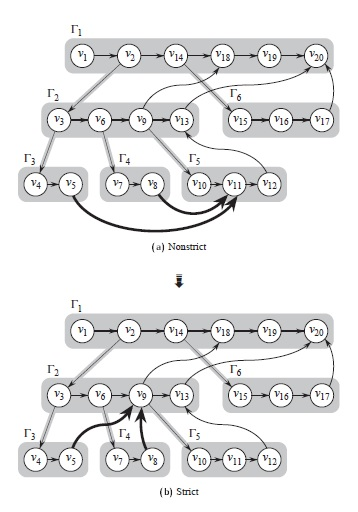
\includegraphics [width=1\linewidth]{img/dagcompare.jpg}
	\caption{Comparison between strict and non-strict DAGs. Accredited to PhD Thesis by Robert D. Blumofe \citep{id13}}
	\label{strictdag}
\end{figure}

\subsubsection{A Unified Scheduler}
\label{section:swan}

The scheduler which this research is focused on is the Swan scheduler. Swan combines work-first scheduling (the approach which Cilk adopts) with dependency-aware scheduling (as seen in SMPSs).

Swan's language is similar to Cilk and the dependency aspect of the scheduler is realised at the object level. The concept of a versioned object is introduced here. 
\begin{comment}
A versioned object is a type of hyper object, allowing all of the meta-data required for dependency tracking to be held at the object level. Included with this is the ability to automatically rename objects to increase task parallelism. 
\end{comment}
These objects are passed to tasks as`indep', `outdep' and `inoutdep' arguments depending on their memory access type. These are defined if a given argument has a memory access mode of: input, output or input/output for a task. If a task has no dependency information associated with it, it is run as an unconditional spawn and is executed as it would be with Cilk.

\begin{comment}
This method of dependency tracking has an added benefit when compared to Cilk in that it records the memory footprint of the tasks. This is useful as it allows for better data locality analysis, this will prove very useful in the tool I hope to create.


Because storing the entire DAG would be expensive in terms of time and memory, Swan uses a ticketing system, based on memory accesses, to correctly sequence tasks that operate on the same objects. The ticket scheduling operates on an object level and each object has 4 counters: a read global counter, a read next counter, a write global counter and a write next counter. These counters work much the same way as a ticketing system at a butcher's shop. Each customer takes a number upon arrival. This updates the `global' counter. So if the first person into the shop got a ticket with the number 15 on it the next person would take a ticket number 16. As the butcher completes an order the `next' counter is incremented inviting the person with the corresponding ticket number to collect their order. Similarly Swan provides tasks with a `ticket' telling them when they can next read or write to a given object. To extend this to the world of parallel programming Swan allows two tasks to have the same ticket number allowing them to execute in parallel. Figure\,\ref{tickettable} gives a summary of the operations on tickets. The R tickets track readers while the W tickets track writers.

\begin{figure} [tp]
	\centering
	\includegraphics [width=1\linewidth] {tickettable.jpg}
	\caption{Reader and writer ticket actions for enqueuing and dequeueing a task and for checking readiness. The operations shown concern one accessed object per task. They are repeated for all arguments of a task, using each respective argument's R and W tickets. The w and r tickets are stored in the task descriptor \citep{id2}.}
	\label{tickettable}
\end{figure}

Let’s study this table for a moment. If we imagine we have a task which wants to read from an object i.e. it has an input dependency on that object. It is strictly queued in the reader set as the read next counter is incremented on enqueue and the read global counter is incremented on dequeue. You will notice however that the ready state of the task doesn't depend on the reader counters. This is because that a reader is not dependent on other readers just on the fact that all previous writers have finished writing to the object. This is why on enqueue the task copies (note it doesn't increment the counter) the next write ticket and is set to ready when the global write counter has reached that write next value. 
\end{comment}

The swan scheduler allows nesting of fork/join parallelism and task graph parallelism. As well as task graphs which are arbitrarily nested. Nested task graphs require care because if the same object is being referenced by both a parent and a child the versioned object meta-data must track the correct dependencies. Swan handles this by creating new counters in the child's object so that dependencies are tracked independently.

\subsection{Scheduler Analysis}

The aim of this research is to analyse parallel schedulers so I will now describe the most relevant work which has been done in this area. There are several analysing tools for parallel systems and the majority follow a similar process which debugs and analyses a post-mortem parallel program. This process is:

\begin{enumerate}
	\item
		\emph{Data collection :} Software is used to collect information about the execution of the parallel program (hardware can be used too).
	\item
		\emph{Data analysis :} Once the stream of events is collected, the analysis step can be started to order, filter, calculate some statistics or simulate a parallel machine.
	\item
		\emph{Display :} Visualise the result provided by the analysis step. 
\end{enumerate}

I will look at each of the scheduler analysing tools in terms of these three areas.

\subsubsection{General Parallel Program Analysis}
There have been tools developed which can analyse the execution trace of a given parallel scheduler. Paraver is such a tool, it visualises parallel execution and displays it in a customisable way. Paraver looks at the actual execution time as a basis of its analysis.  It uses various windows to display information to the user all of which is customisable so the user can view the collection of windows which most suits their purpose. These update as the user traces through the program, representing what is happening through various views. The ability to filter and to vizualise execution is useful however a lot of effort is required from the user in order to get a meaningful metric to help them improve their application. Paraver is also only interested in the display aspect of the analysis process. The data collection and exporting have to be applied to the program before Paraver is able to display it from a simulation file. This collection is very expensive and collecting a trace file can slow a runtime system down by an order of magnitude - leaving the user with an inaccurate measurement.

\subsubsection{Work First Analysis}
\label{section:cilkview}

Cilkview is an analysing tool for Cilk which is useful to this research because Swan extends Cilk and benefits from much of the same analysis.

Cilkview first collects a program's parallelism information during a serial execution of the program code. It uses meta data in Cilk++ to identify the parallel control constructs in the executing application which allows it to construct a data dependency DAG. As this meta data is built into the Cilk++ binary it imposes no overhead on performance in a normal production environment. Instead of capturing exact timing measurements Cilkview uses instruction count as a surrogate of time. They feel that parallelism estimates accurate to within a binary order of magnitude suffice to diagnose problems of inadequate parallelism. 

Cilkview focuses on three areas when analysing the results from \emph{work, span and burdened span}. I will look at how each of these are calculated in turn and discuss why they are important. 

Work is the total amount of time spent in all the strands. Let \(T_P\) be the fastest possible execution time of the application on \(P\) processors. Since the work corresponds to the execution time on 1 processor, we denote it by \(T_1\). One reason that work is an important measure is that it provides a lower bound on P-processor execution time: 

\[T_P \geq T_1/P\]

This is at least how much time it takes for \(P\) processors to execute the total amount of work done. Because theoretically \(P\) processors can do \(P\) instructions at one time. Using Cilk \(T_1/T_P\) is the most \emph{speedup} that can be gained. Speedup is how much faster a program can run on a given environment this can be intuitively written as a program which is run on a machine with 5 processors can run 5 times as fast. This level of speedup is known as linear speed up.

The second area which Cilkview analyses is span. Span is also called the critical path and is the longest amount of time which is taken for a program to execute over any path of dependencies in the DAG. The critical path is the theoretical fastest time which a program could be run on an unlimited amount of processors. Due this it is denoted as \(T_\infty\) this also provides a bound on \(P\) processor execution time:

\[T_P \geq T_\infty\]

Cilkview uses the work and span to calculate the parallelism of a program \(T_1/T_\infty\). The parallelism is the average amount of work along each step of the critical path. From parallelism we can work out what the maximum number of processors are on which linear speed-up can be achieved for a particular program. Linear speed-up cannot be achieved on any number of processors greater than the parallelism. This information allows Cilkview to determine how scalable a program is. 

The third aspect which Cilkview analyses is the burdened span. Although the execution time is reduced by tasks being run on various processors the overhead and book-keeping which is introduced to schedule these executions needs to be taken into account. This is what the burdened DAG does. In Cilkview a constant called the \emph{span coefficient} \(\delta\) is multiplied by the span to take into account the work stealing overhead which includes the book keeping and the cost of cache misses in order to migrate the stolen task's working set.

\[T_P \leq T_1/P+\delta T \infty\]

The burdened DAG places a burden on each continuation and return edge of the DAG. Cilkview computes the \emph{burdened span} by finding the longest path in the burdened DAG. 

If we let \(T_1\) be the work of an application program, and let \(\hat{T}_\infty\) be its burdened span. Then, a work-stealing scheduler running on \(P\) processors can execute the application in expected time:

\[T_P \leq T_1 / P+2 \delta \hat{T}_\infty\]

Cilkview uses this burdened model to give a more accurate estimated lower bound on speedup. This is, a work-stealing scheduler running on P processors achieves speedup at least:

\[\frac{T_1}{T_P}\geq\frac{T_1}{T_1/P+2 \delta \hat{T}_\infty}\]

A detailed proof of this can be found in Cilkview's research paper \citep{id8}.

Cilkview displays the following information to the user: amount of work done, the span, the burdened span, the parallelism, the burdened parallelism, number of spawns, number of syncs and the average maximal strand (which is how much work is down in between scheduler operations). Cilkview then gives estimated speedups for 2 - 32 processors. Cilkview also uses graphs to display this data in a meaningful way.

\begin{comment}
Although Cilkview provides excellent scalability information it doesn't give an analysis of memory management or time taken for tasks. It may be useful to know if a larger cache would be of use to your program and if so to what extent. Also instruction count may not be an accurate enough measure of work when a user is really interested in the time taken to run and schedule a task. 

\subsubsection{Data Locality}
One area that hasn't been discussed yet is the idea of memory access between threads. SMPSs did consider this by attempting to schedule serial instructions to one processor but the effectiveness of this is questionable. There are other models which are able to analyse how the order in which tasks are scheduled effects a shared cache \citep{id12}. This can have a positive or negative effect. On the negative size if two threads are working on completely different data and accessing the same cache \(T_1\) will place its working set on the cache closest to the processor which means when \(T_2\) needs to access its working set it will have to look deeper into the cache or even into the main memory to retrieve its information. On the other hand, if the two treads are working on the same data \(T_1\) may actually shorten the distance of data from \(T_2\) when \(T_2\) goes to use it next. There has been successful research into predicting how shared memory will be used between threads and tools have been developed to capture such information an example of which being Cache Pirate \citep{id17}. It has been shown \citep{id21} that a 15 - 60\% improvement of run time can be achieved by taking data locality into account.
\end{comment}

\subsection{Other Metrics}
There are other metrics which have been used to measure the performance of parallel applications, examples of these are: True Zeroing\citep{id20}, Gprof\citep{id18} and Quartz NPT\citep{id19}. An overall study and comparison of each method has been carried out \citep{id4} and suggests that critical path analysis, as discussed in section \ref{section:cilkview}, is most effective.

\begin{comment}
\section{Methods To Be Used}

\subsubsection{Task Dependencies}
I will need to record the task dependency graph in order to analysis things like the critical path (or span) which, as we've seen, can be used to produce a lot of valuable information. I will have to ensure that I do it in a way which is inexpensive in terms of time and memory as this could skew the reporting. I hope to use the information that swan already uses i.e. the memory access type of each task to a specific object in order to build the DAG at the post-processing stage. This is in-line with the approach that Cilkview adopted by using Cilk++'s meta data. They have been able to show that it has virtually no effect on the performance of the program and I hope to achieve the same.

\subsubsection{Timing}
I will also look into recording the amount of time elapsed as done in analysis tools such as Paraver. This could prove useful as execution time is likely to be the most important result of parallelising an application to the user. For each task Paraver records the start time and end time and then works out the elapsed time in post processing. I will need to see how this would impact the running of Swan if I was to implement this additional recording. It may be sufficient to work out an average time per task and per scheduling instruction in post processing using fewer time stamps combined with a count of the number of tasks and scheduling operations between the two time stamps. 

\subsubsection{Data Locality}
Memory management is the third thing that I hope to analyse. I will need to discover the amount of memory which is available to each processor and if this memory is shared who is it shared with. I will then need analyse how the amount of memory available to a processor effects the execution of a sequence of tasks. If this has a sufficient amount of impact I will investigate if it is possible to arrange the tasks in a way which will maximise the memory available.

There is potential for this to be done by executing tasks which require complementing proportions of cache memory to processors which share cache. For example if tasks \(T_1\) and \(T_2\) both access the same data then scheduling them to run on \(P_1\) and \(P_2\) would yield benefits as described in Section \ref.

If this is not achievable another method which could maximise the use of available memory is if task \(T_3\) requires 60\% of a cache's space and task \(T_4\) requires 40\% they should be scheduled on processors \(P_1\) and \(P_2\) provided that these processors share the same cache.

Once I have determined if these are possible I will analyses how much difference a more efficient arrangement would make to program execution. We have been given access and permission to use cache pirate's (introduced in Section 2.2.3) source code which could prove useful in gaining this information.

I will be able to get an estimate of how much memory a task will use by looking at the footprint which can be extracted by how Swan requires the programmer to define task dependencies.

\section{Expected Results}

My overall result will be a tool which is able to effectively analyses a parallel program that combines task data flow dependency tracking with a work-first scheduling approach. The tool should produce accurate and helpful results in areas such as parallelism, critical path analysis, memory locality and elapsed time. Each of these have been analysed in various tools in the past but right now there is no solution which can combine the advantages of all of these.  This should lead to more efficient parallel programs whether that's through understanding how to create better programs or making improvements to the scheduler. 
\end{comment}